% "Станет проще"

\documentclass[a4paper,12pt]{article} % тип документа

% report, book

%  Русский язык

\usepackage[T2A]{fontenc}			% кодировка
\usepackage[utf8]{inputenc}			% кодировка исходного текста
\usepackage{graphicx}
\usepackage[english,russian]{babel}	% локализация и переносы



\usepackage[left=10mm, top=10mm, right=10mm, bottom=10mm, nohead, nofoot]{geometry}
% Математика
\usepackage{amsmath,amsfonts,amssymb,amsthm,mathtools} 
\usepackage{csvsimple}
\usepackage{multirow}


\usepackage{wasysym}
\usepackage{subcaption}
\usepackage{gensymb}
\usepackage{verbatim}
\usepackage[hidelinks]{hyperref}
\usepackage{float}
\usepackage{enumerate}
\usepackage{wrapfig}
\usepackage{listings} %написание кода
%\usepackage{fancyhdr}

\usepackage[dvipsnames]{xcolor}
\usepackage{verbatim} %comments

%Заговолок



\graphicspath{ {img/} }


\begin{titlepage}
\author{Соловьянов Михаил}
\title{Введение в цифровую элекронику}
\date{\today}
\end{titlepage}


\begin{document}
\thispagestyle{empty}


\includegraphics[width=3.5cm]{logo.png} \ \large {Введение в цифровую электронику. Мастер-класс. \today}



\section{Вентили}




\begin{table}[H]
\centering
\begin{tabular}{|l|l|l|l|l|l|l|l|l|l|l|}
\cline{1-3} \cline{5-7} \cline{9-11}
\multicolumn{3}{|l|}{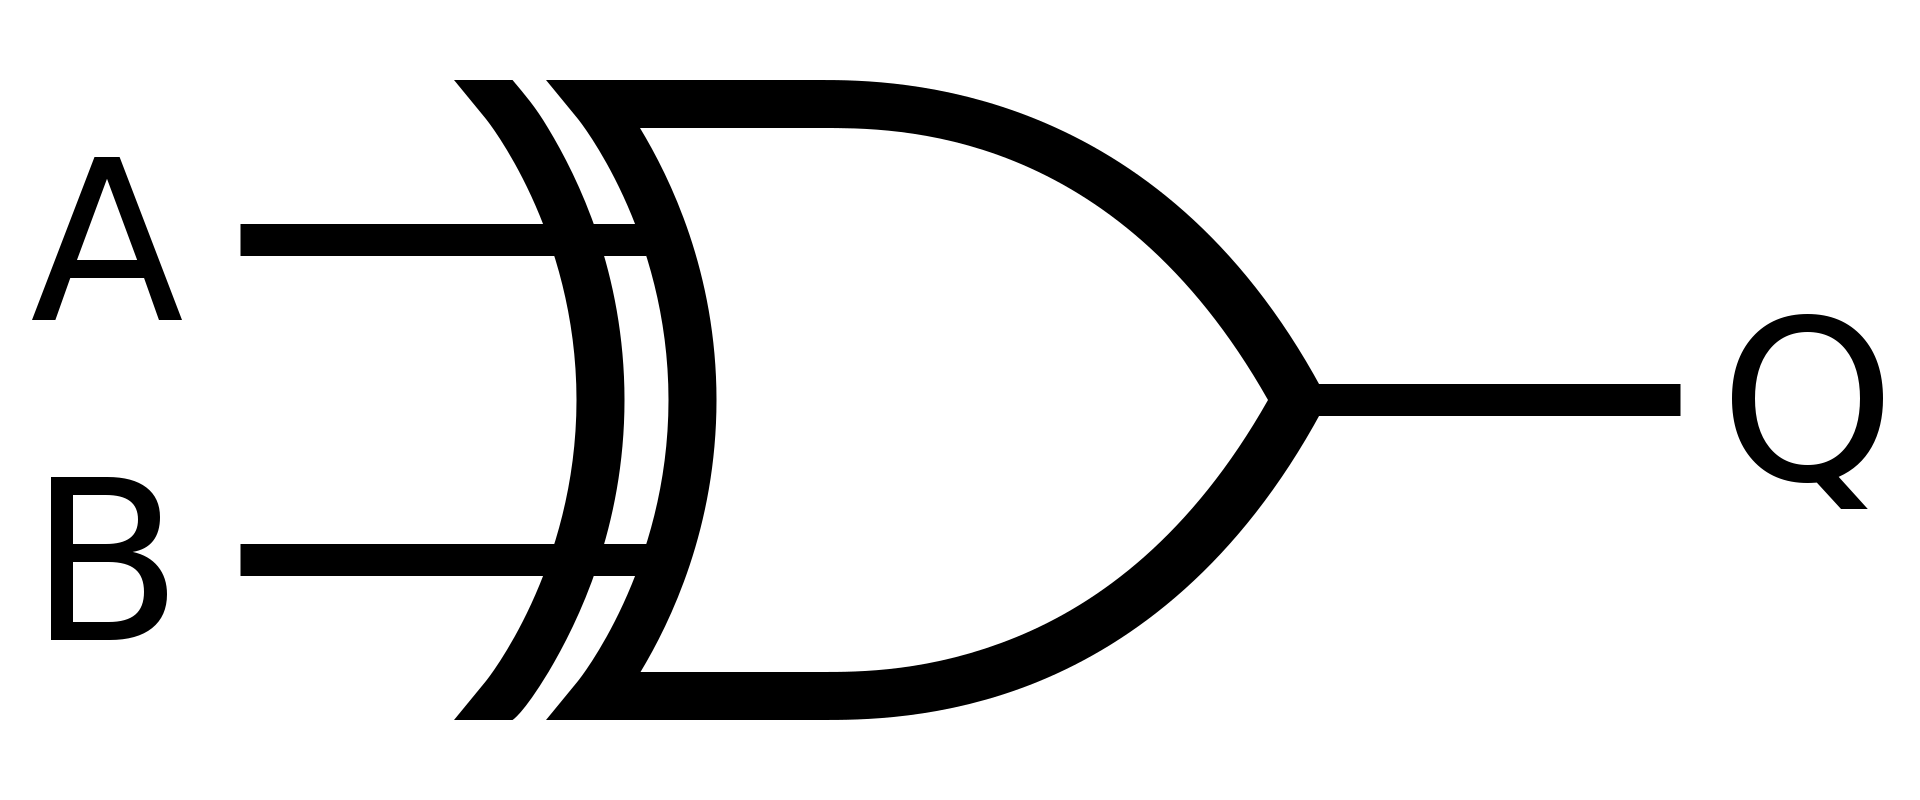
\includegraphics[width=1.1cm]{or_true.png}} &  & \multicolumn{3}{l|}{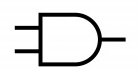
\includegraphics[width=1.1cm]{and.jpg}}  &  & \multicolumn{3}{l|}{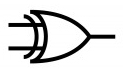
\includegraphics[width=1.1cm]{xor.jpg}}  \\ \cline{1-3} \cline{5-7} \cline{9-11} 
$ A  $      & $B$      &$ A+B $     &  &$ A  $    & $B$      & $A \times B$     &  &$ A  $       & $B$      & $A \oplus B$     \\ \cline{1-3} \cline{5-7} \cline{9-11} 
1      & 0      & 1        &  & 1      & 0      & 0       &  & 1      & 0      & 1       \\ \cline{1-3} \cline{5-7} \cline{9-11} 
0      & 1      & 1        &  & 0      & 1      & 0       &  & 0      & 1      & 1       \\ \cline{1-3} \cline{5-7} \cline{9-11} 
0      & 0      & 0        &  & 0      & 0      & 0       &  & 0      & 0      & 0       \\ \cline{1-3} \cline{5-7} \cline{9-11} 
1      & 1      & 1        &  & 1      & 1      & 1       &  & 1      & 1      & 0       \\ \cline{1-3} \cline{5-7} \cline{9-11} 
\end{tabular}
\end{table}


\section{Двоичное исчисление}
\large{
$1_2 + 1_2 = 10_2 $\\
$1111_2 = 2^3 + 2^2 + 2^1 + 2^0 = 8 + 4 +2 +1 =15 $
}




\section{Микросхемы}

\begin{minipage}{0.45\textwidth}

\begin{center}


 \Large { MM74HCT08N}

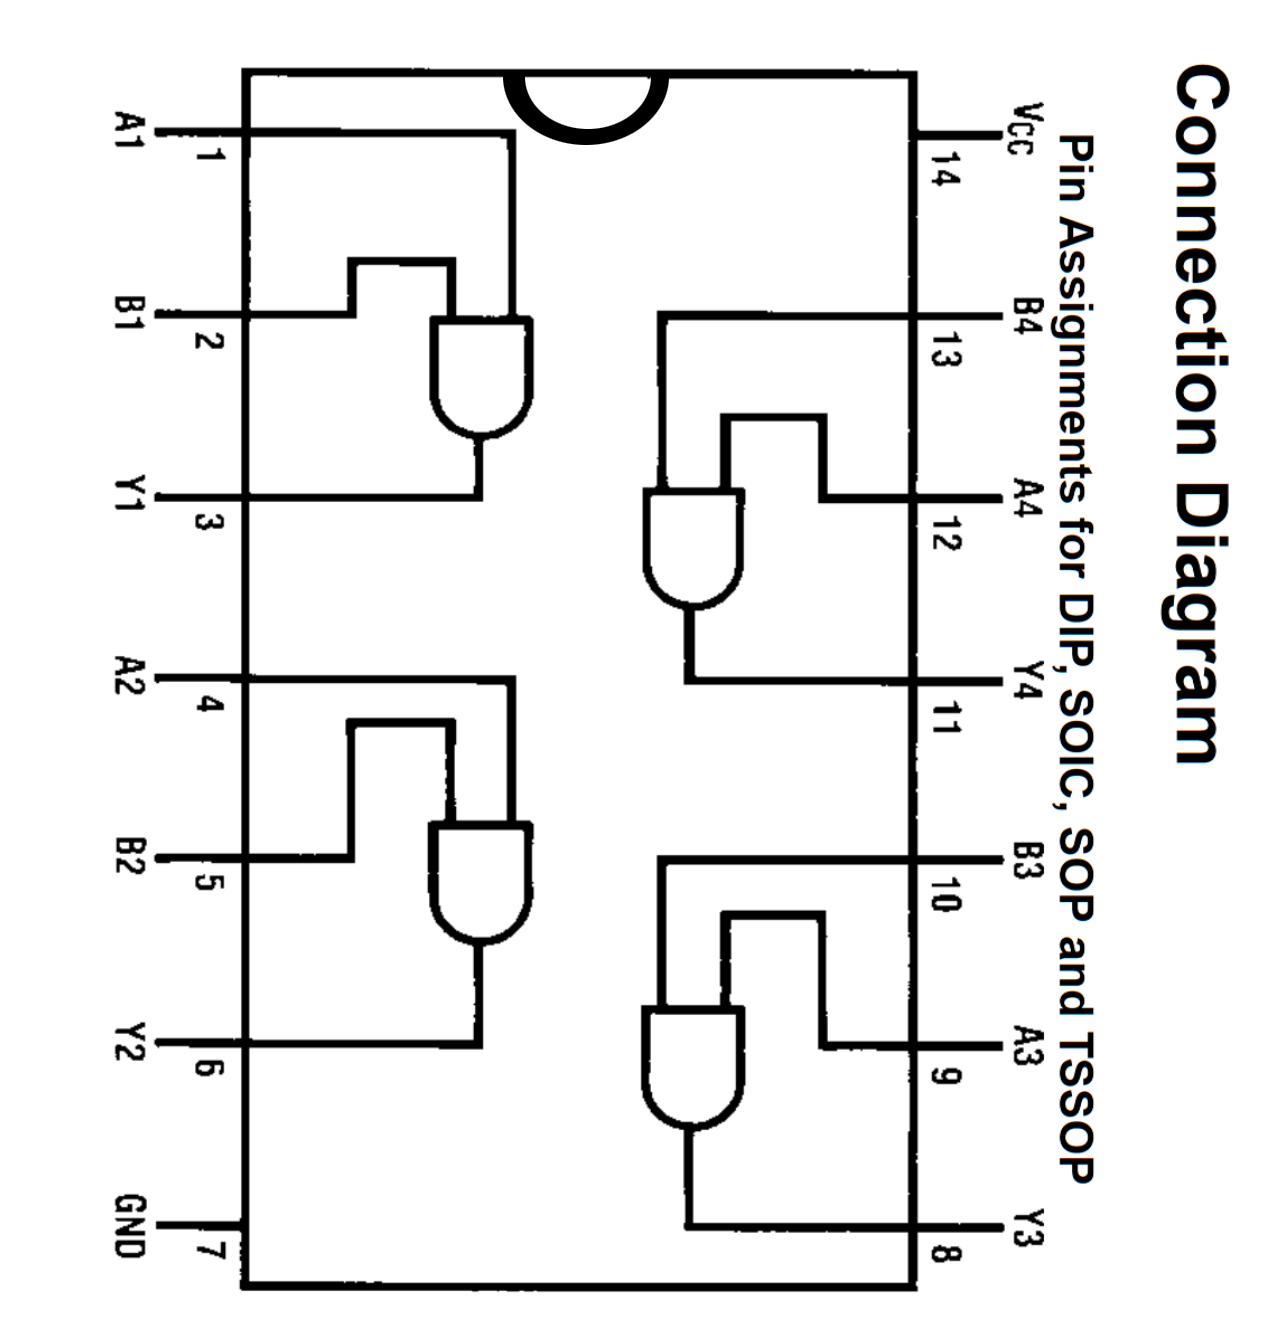
\includegraphics[width=7cm]{sc.png}\\


\end{center}

\end{minipage}%
\hfill
\begin{minipage}{0.45\textwidth}
\begin{tabular}{|p{\textwidth}}




\begin{center}
 \LARGE {SN74HC86N}

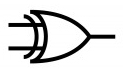
\includegraphics[width=5.6cm]{xor.png}

\LARGE{$Y = A \oplus B $} \\
\vspace{0.5cm}

\end{center}

\end{tabular}
\end{minipage}%


\section{Сумматор}


\begin{minipage}{0.5\textwidth}

\begin{center}

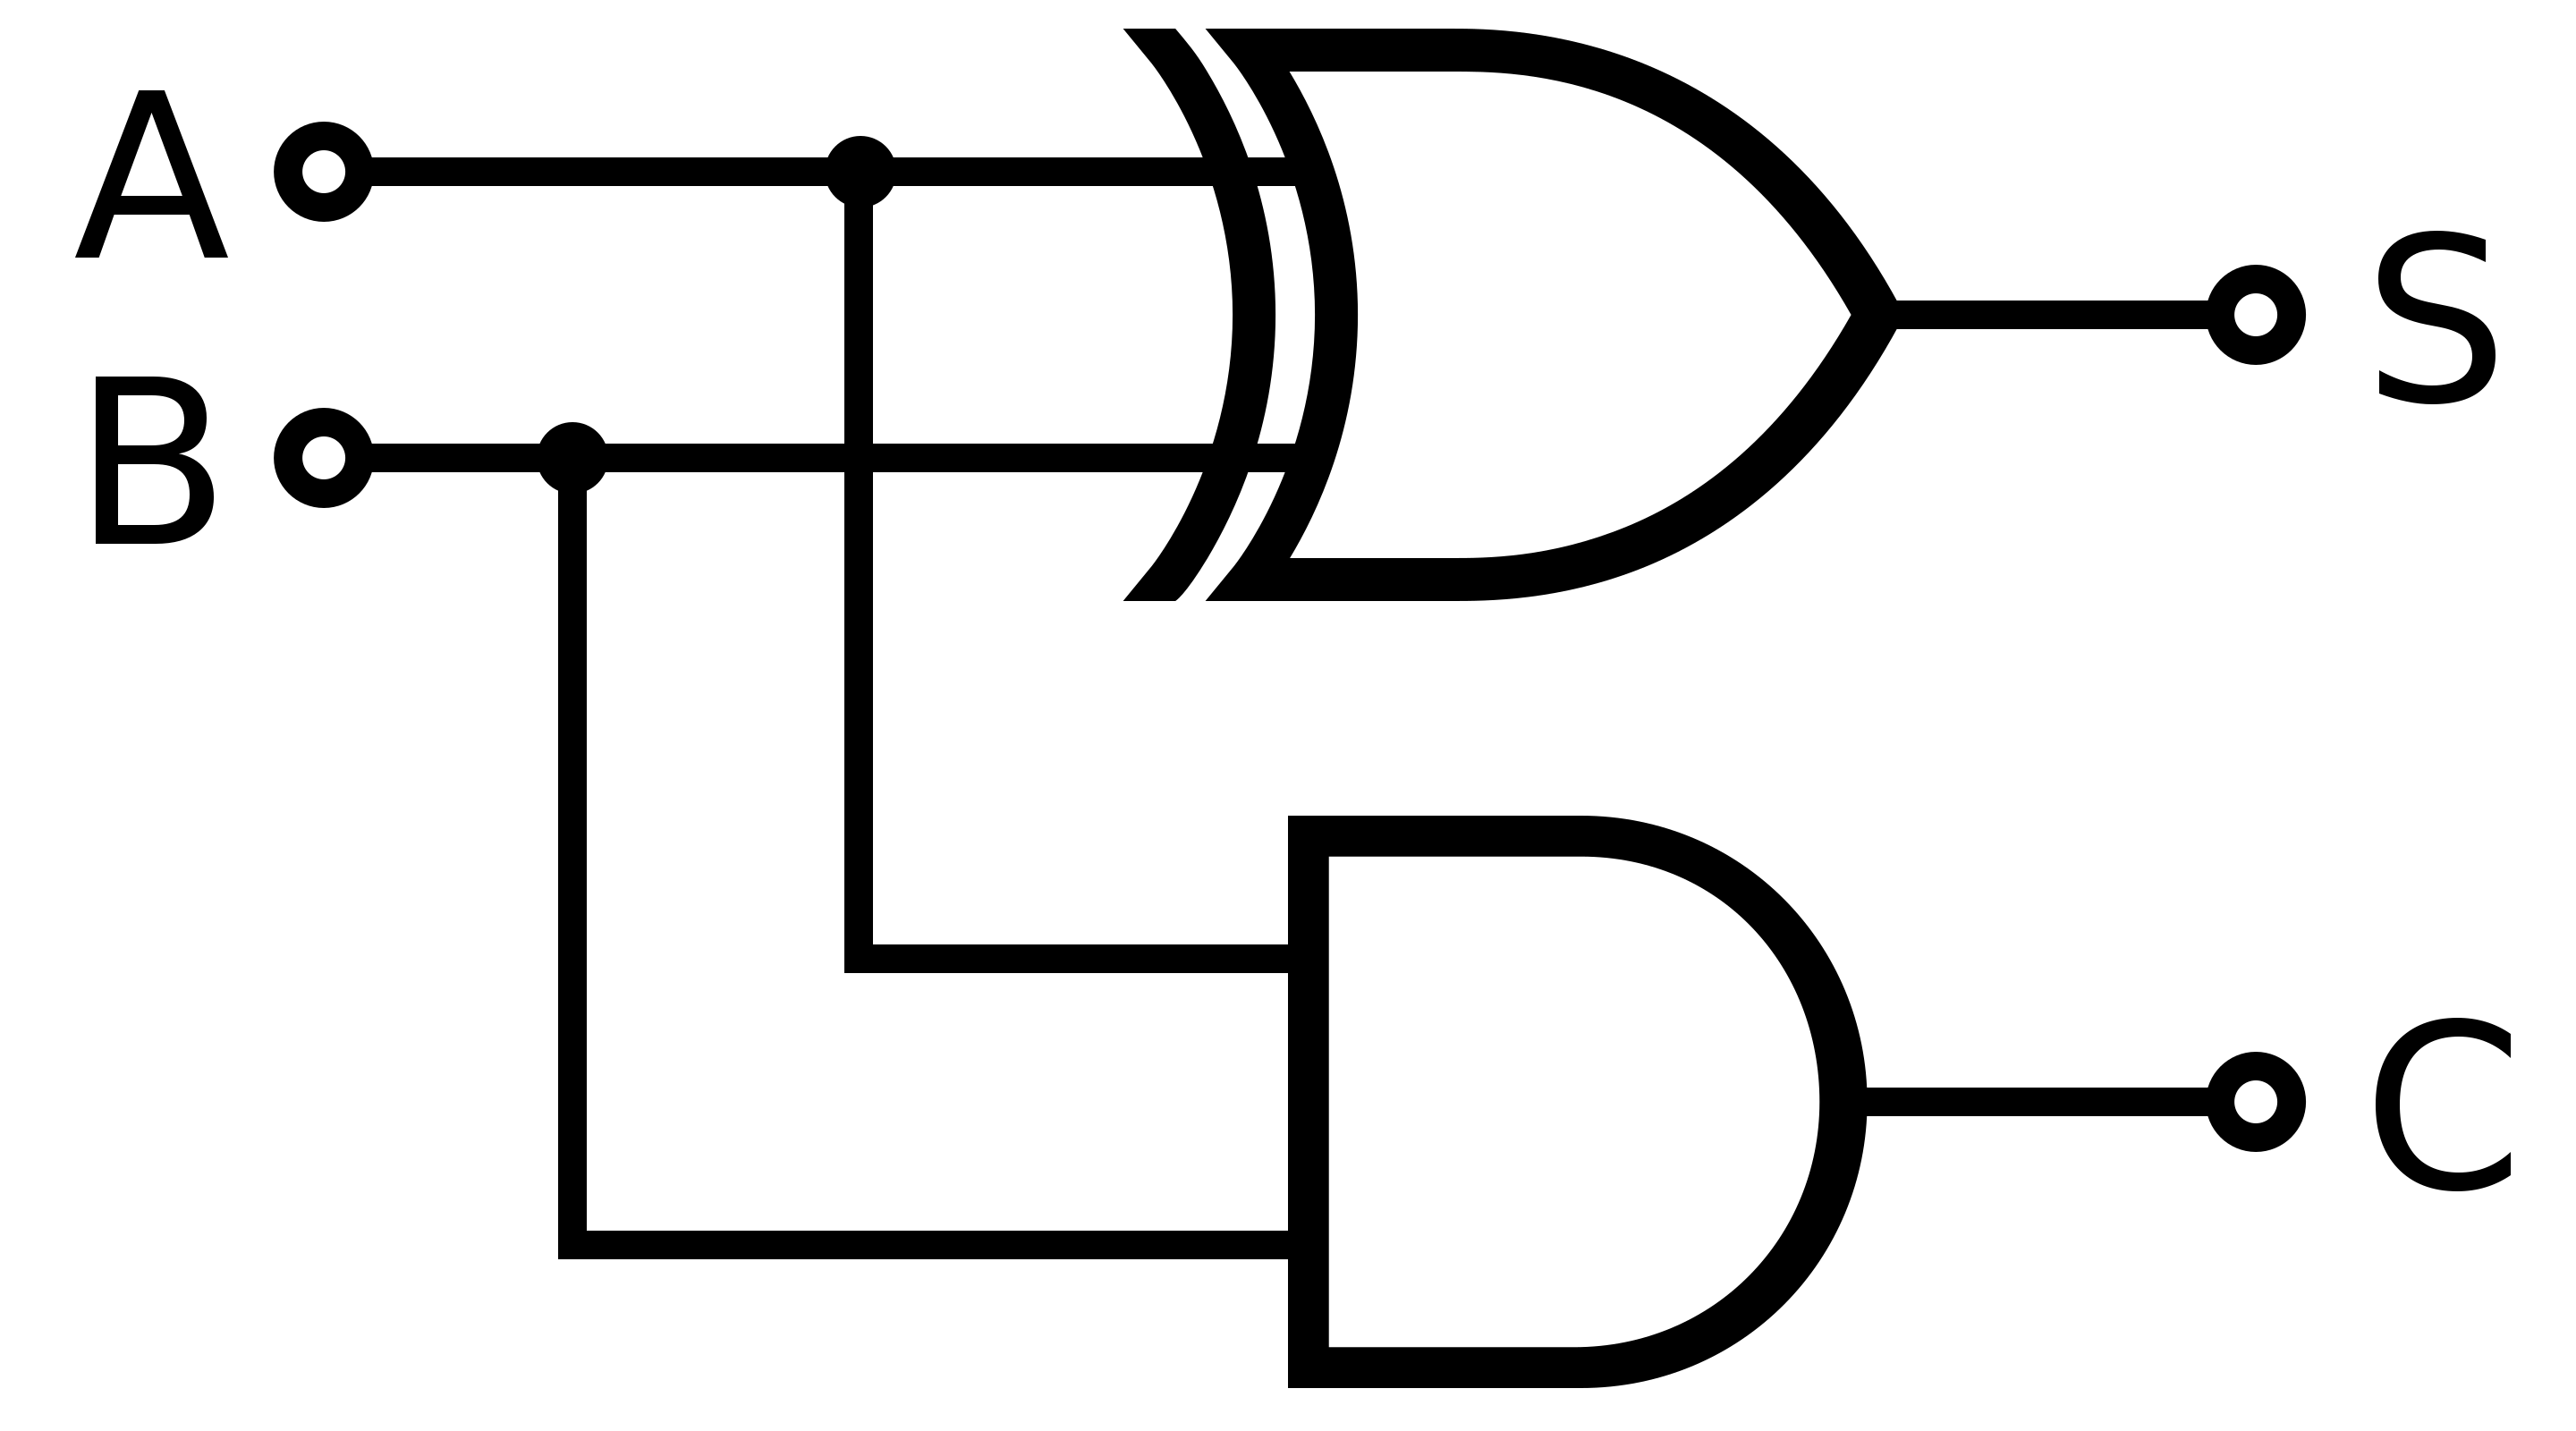
\includegraphics[width=\textwidth]{h_adder.png}\\

Схема полу-сумматора предлагаемого к сборке на мастер классе
\end{center}
\end{minipage}%
\hfill
\begin{minipage}{0.40\textwidth}
\begin{tabular}{|p{\textwidth}}




\begin{center}

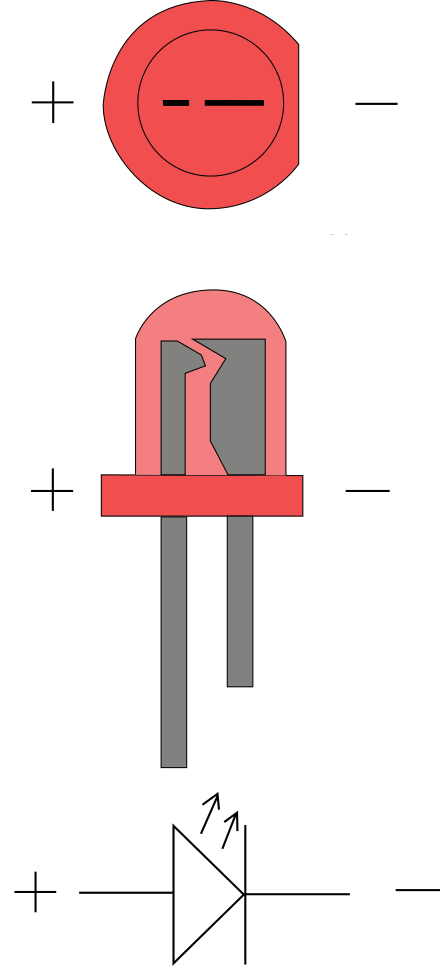
\includegraphics[width=3cm]{diode.png}\\
Определение полярности диода.
\end{center}

\end{tabular}
\end{minipage}%
\begin{center}
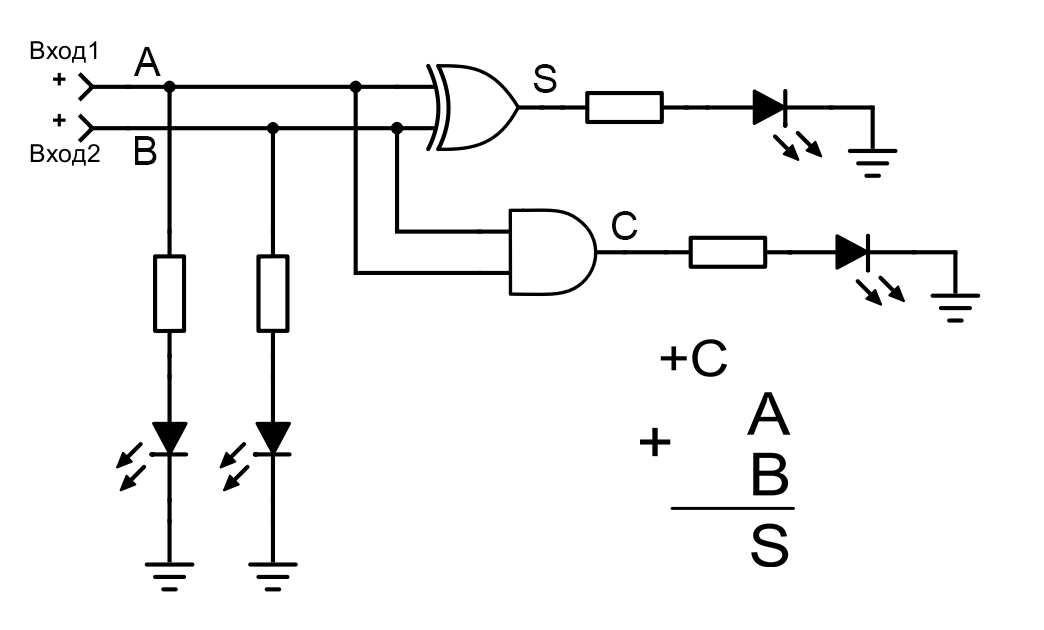
\includegraphics[width=\textwidth]{project.png}\\
Полная схема необходимая к сборке.

\end{center}















\end{document}
